\chapter{Resultados e Discussão}\label{cap:resultados}

Após entender o funcionamento do algoritmo de Viola Jones, foram executados testes com os conjuntos de imagens selecionados e os resultados obtidos são discutidos a seguir.

Inicialmente, foi necessário especificar com clareza como poderiam ser agrupadas as imagens, dada a sua origem e o resultado observado no teste, para isso foram utilizadas as definições da tabela \ref{tab:grupos-images}. 

\begin{table}[htbp]
    \caption{Grupos observados}
    \label{tab:grupos-images}
    \centering
    \begin{tabular}{ccc}\hline\hline
        \textbf{Grupo} & \textbf{Descrição} & \textbf{Quantidade} \\\hline
        \textit{A} & Imagens que não contêm nenhuma face & 17130 \\
        $\overline{A}$ & Imagens que contêm uma face & 17130 \\
        \textit{B} & Imagens onde o algoritmo não identificou nenhuma face & Variável \\
        $\overline{B}$ & Imagens onde o algoritmo identificou uma ou mais faces & Variável \\
    \hline\hline
    \end{tabular}
\end{table}

Definidos os grupos, pode-se utilizar a tabela de contingência \ref{tab:tabela_contingencia} para facilitar a análise da relação entre os grupos definidos anteriormente. Na tabela \ref{tab:tabela_contingencia} são observados os grupos \textit{a} (verdadeiro positivo) onde o algoritmo identifica corretamente uma face em cada uma das imagens que realmente contêm uma face, \textit{b} (falso negativo) onde o algoritmo erroneamente não reconheceu nenhuma face, apesar das imageens conterem uma face cada, \textit{c} (falso positivo) onde o algoritmo erroneamente identificou ao menos uma face, mesmo as imagens não contendo nenhuma e \textit{d} (verdadeiro negativo) onde o algoritmo identificou corretamente que não existia nenhuma face nas imagens. É importante destacar que os quatro grupos destacados na tabela de contingência são mutuamente excludentes. \cite{Dougherty:2012:PRC:2553126}

\begin{table}[htbp]
    \caption{Tabela de contingência}
    \label{tab:tabela_contingencia}
    \centering
    \begin{tabular}{ccc}\hline\hline
        & \textit{B} & $\overline{B}$ \\
    \textit{A} & \textit{a} (verdadeiro positivo) & \textit{b} (falso negativo) \\
    $\overline{A}$ & \textit{c} (falso positivo) & \textit{d} (verdadeiro negativo) \\
    \hline\hline
    \end{tabular}
\end{table}

Para melhor entender os agrupamentos da tabela de contingência, pode-se observar na imagem \ref{fig:norm_dist} as distribuições que representam a quantidade de imagens dos grupos \textit{A} e $\overline{A}$ dada a sua probabilidade de conter uma face. 

\begin{figure}[htbp]
    \centering
    \caption{Possível distribuição normal dos grupos observados na tabela de contingência.}
    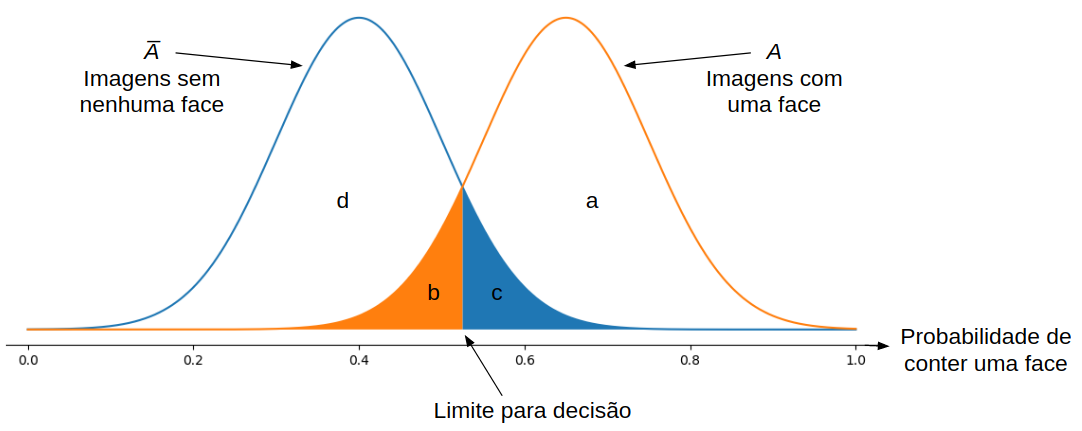
\includegraphics[scale=.5]{figs/norm_dist.png}
    \label{fig:norm_dist}
 \end{figure}

 Nas distribuições são destacados os grupos \textit{b} (falso negativo) e \textit{c} (falso positivo) e fica evidente que, devido a sobreposição das distribuições \textit{A} e $\overline{A}$, é necessário definir uma limite para decisão, que pode ser ajustado conforme a necessidade, mas que independente do seu ajuste, sempre existirá um grupo categorizado de forma incorreta.

 A tabela de contingência também pode ser escrita em termos probabilísticos (tabela \ref{tab:tabela_contingencia_probab}), incluindo as probabilidades marginais ou pode ser visualizada no diagrama de Venn correspondente (figura \ref{fig:venn_diagram}).

\begin{table}[htbp]
    \caption{Tabela de contingência com probabilidades marginais}
    \label{tab:tabela_contingencia_probab}
    \centering
    \begin{tabular}{cccc}\hline\hline
        & \textit{B} & $\overline{B}$ & Soma\\
    \textit{A} & $P(A \cap B)$ & $P(A \cap \overline{B})$ & $P(A)$ \\
    $\overline{A}$ & $P(\overline{A} \cap B)$ & $P(\overline{A} \cap \overline{B})$ & $P(\overline{A})$ \\
    Soma & $P(B)$ & $P(\overline{B})$ & 1 \\
    \hline\hline
    \end{tabular}
\end{table}

 \begin{figure}[htbp]
     \centering
     \caption{Diagrama de Venn para as imagens analisadas.}
     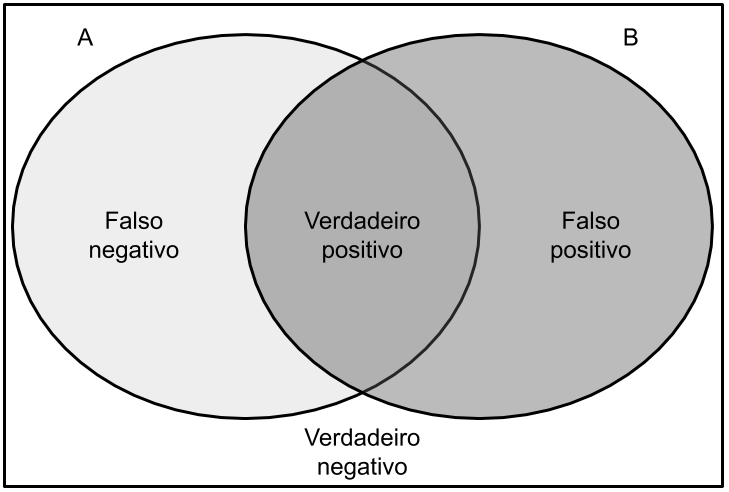
\includegraphics[scale=.4]{figs/venn-diagram.png}
     \label{fig:venn_diagram}
  \end{figure}

Por fim, podem ser calculadas as medidas tradicionais de sensitividade (a probabilidade condicional do algoritmo identificar ao menos uma face dado que a imagem contém uma face) e especificidade (a probabilidade condicional do algoritmo não identificar nenhuma face em uma imagem que realmente não contém nenhuma face) conforme as equações \ref{eq:sensitividade} e \ref{eq:especificidade}.

\begin{equation} \label{eq:sensitividade}
    \text{sensitividade, } P(B|A) = P(A \cap B) / (P(A \cap B) + P(A \cap \overline{B})) = a/(a + b)
\end{equation}

\begin{equation} \label{eq:especificidade}
    \text{especificidade, } P(\overline{B} | \overline{A}) = P(\overline{A} \cap \overline{B}) / (P(\overline{A} \cap \overline{B}) + P(\overline{A} \cap B)) = d/(d + c)
\end{equation}

A biblioteca OpenCV permite ainda ajuste de alguns parâmetros para a execução do algoritmo de Viola Jones, no primeiro teste executado sobre o conjunto de imagens, foram configurados os parâmetros de fator de escala para 1.3 e número mínimo de vizinhos para 5, após analisar todas imagens foi possível preencher a tabela de contingência \ref{tab:tabela_contingencia_teste1} e calcular a respectiva sensitividade $P(B|A) = 98.5872\%$ e especificidade $P(\overline{B} | \overline{A}) = 86.6024\%$.

\begin{table}[htbp]
    \caption{Tabela de contingência com os resultados do primeiro teste}
    \label{tab:tabela_contingencia_teste1}
    \centering
    \begin{tabular}{cccc}\hline\hline
        & \textit{B} & $\overline{B}$ & Soma\\
    \textit{A} & 49.2936\% & 00.7064\% & 50\% \\
    $\overline{A}$ & 06.6988\% & 43.3012\% & 50\% \\
    Soma & 55.9924\% & 44.0076\% & 100\% \\
    \hline\hline
    \end{tabular}
\end{table}

Ajustando o fator de escala para 1.05 e o número mínimo de vizinhos para 3, foram obtidos os resultados apresentados na tabela \ref{tab:tabela_contingencia_teste2} e a respectiva sensitividade $P(B|A) = 66.3923\%$ e especificidade $P(\overline{B} | \overline{A}) = 98.3479\%$.

\begin{table}[htbp]
    \caption{Tabela de contingência com os resultados do segundo teste}
    \label{tab:tabela_contingencia_teste2}
    \centering
    \begin{tabular}{cccc}\hline\hline
        & \textit{B} & $\overline{B}$ & Soma\\
    \textit{A}& 33.1962\% & 16.8038\% & 50\% \\
    $\overline{A}$& 00.8260\% & 49.1740\% & 50\% \\
    Soma& 34.0222\% & 65.9778\% & 100\% \\
    \hline\hline
    \end{tabular}
\end{table}
